\section{Star planet orbiting}
\subsection{Orbiting}
\begin{frame}
\only<1-2>{
	\frametitle{Efficient orbiting using a Finite State Machine (FSM)}
	\only<1->{
		\textbf{Objective:} Algorithm to allow a planet to orbit n stars from any initial condition.
	}
	\begin{itemize}
		\only<1->{
			\item \textbf{Stars:} Stationary bots around which planet rotates (Black)
			\only<2->{
			\item \textbf{Planet:} Dynamic bots rotating around stars (Gray)
			}
		}
	\end{itemize}
			\begin{columns}[b]
			\begin{column}{0.2\textwidth}
				\begin{figure}
					\centering
					\only<1>
					{
					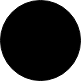
\includegraphics[scale=0.25]{star1}
					}
					\only<2>
					{
						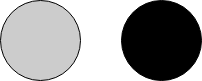
\includegraphics[scale=0.25]{star1planet}
					}
					\vspace{0.4cm}
					\caption{Single star system}
				\end{figure}
			\end{column}
			\begin{column}{0.33\textwidth}	
				\begin{figure}
					\centering
					\only<1>
					{
						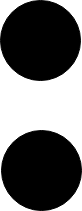
\includegraphics[scale=0.25]{star2}
					}
					\only<2>
					{
						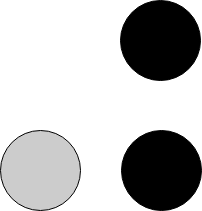
\includegraphics[scale=0.25]{star2planet}
					}
					\vspace{0.4 cm}
					\caption{Linear star system}
				\end{figure}
			\end{column}
			\begin{column}{0.33\textwidth}
				\begin{figure}
					\centering
					\only<1>
					{
						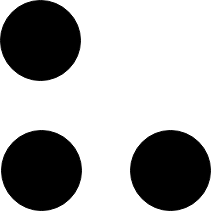
\includegraphics[scale=0.25]{star3}
					}
					\only<2>
					{
						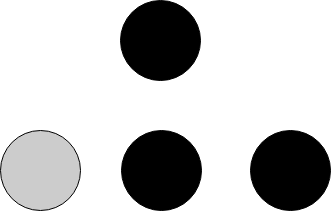
\includegraphics[scale=0.25]{star3planet}
					}
					\hspace{5 cm}
					\caption{Triangular star system}
				\end{figure}
		\end{column}
	\end{columns}
}
\end{frame}

\begin{frame}
\frametitle{Flowchart}
\begin{figure}[H]
	\centering
	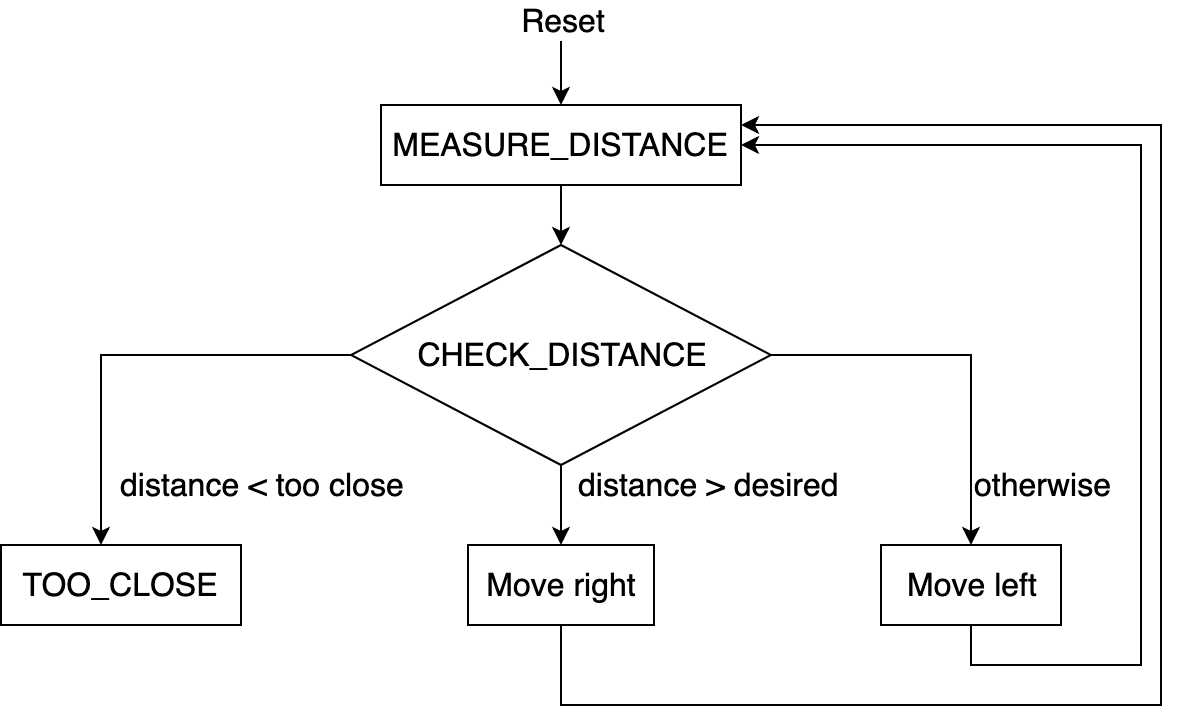
\includegraphics[scale=0.27]{star_planet_escape_compressed_1}
\end{figure}
\end{frame}

\begin{frame}
\frametitle{Efficient orbiting using FSM}
\framesubtitle{Demonstration}
	\begin{figure}[H]
		\begin{center}
		\fbox{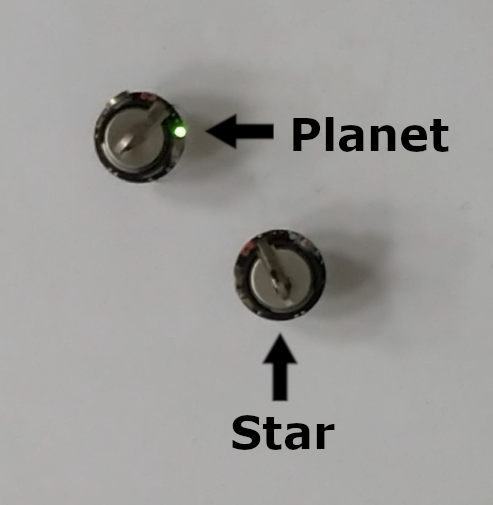
\includegraphics[width=2in]{efficient_orbiting}}\\
		\hspace{5cm}
		\caption{\href{https://youtu.be/LRgOzhAJI1k}{Efficient star-planet orbiting using single communication}}
		\label{fig:shape_formation_demo}
	\end{center}
	\end{figure}
\end{frame}

\subsection{Escaping the close region}
\begin{frame}
\frametitle{Escaping the close region}
\textbf{Objective:} Designing a robust algorithm to reach the desired orbit distance without hitting the star.
\only<2->{
\begin{columns}[b]
	\begin{column}{0.5\textwidth}
		\begin{figure}
			\centering
			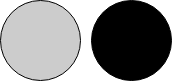
\includegraphics[scale=0.25]{star1planet_close}
			\hspace{5 cm}
			\caption{Planet too close to star}
		\end{figure}
	\end{column}
	\begin{column}{0.5\textwidth}	
		\begin{figure}
			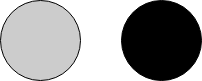
\includegraphics[scale=0.25]{star1planet}
			\hspace{5 cm}
			\caption{Desired distance of orbit}
		\end{figure}
	\end{column}
\end{columns}
}
\end{frame}

\begin{frame}
\frametitle{Snapshots}
	\only<1>{
	\begin{figure}
		\centering
			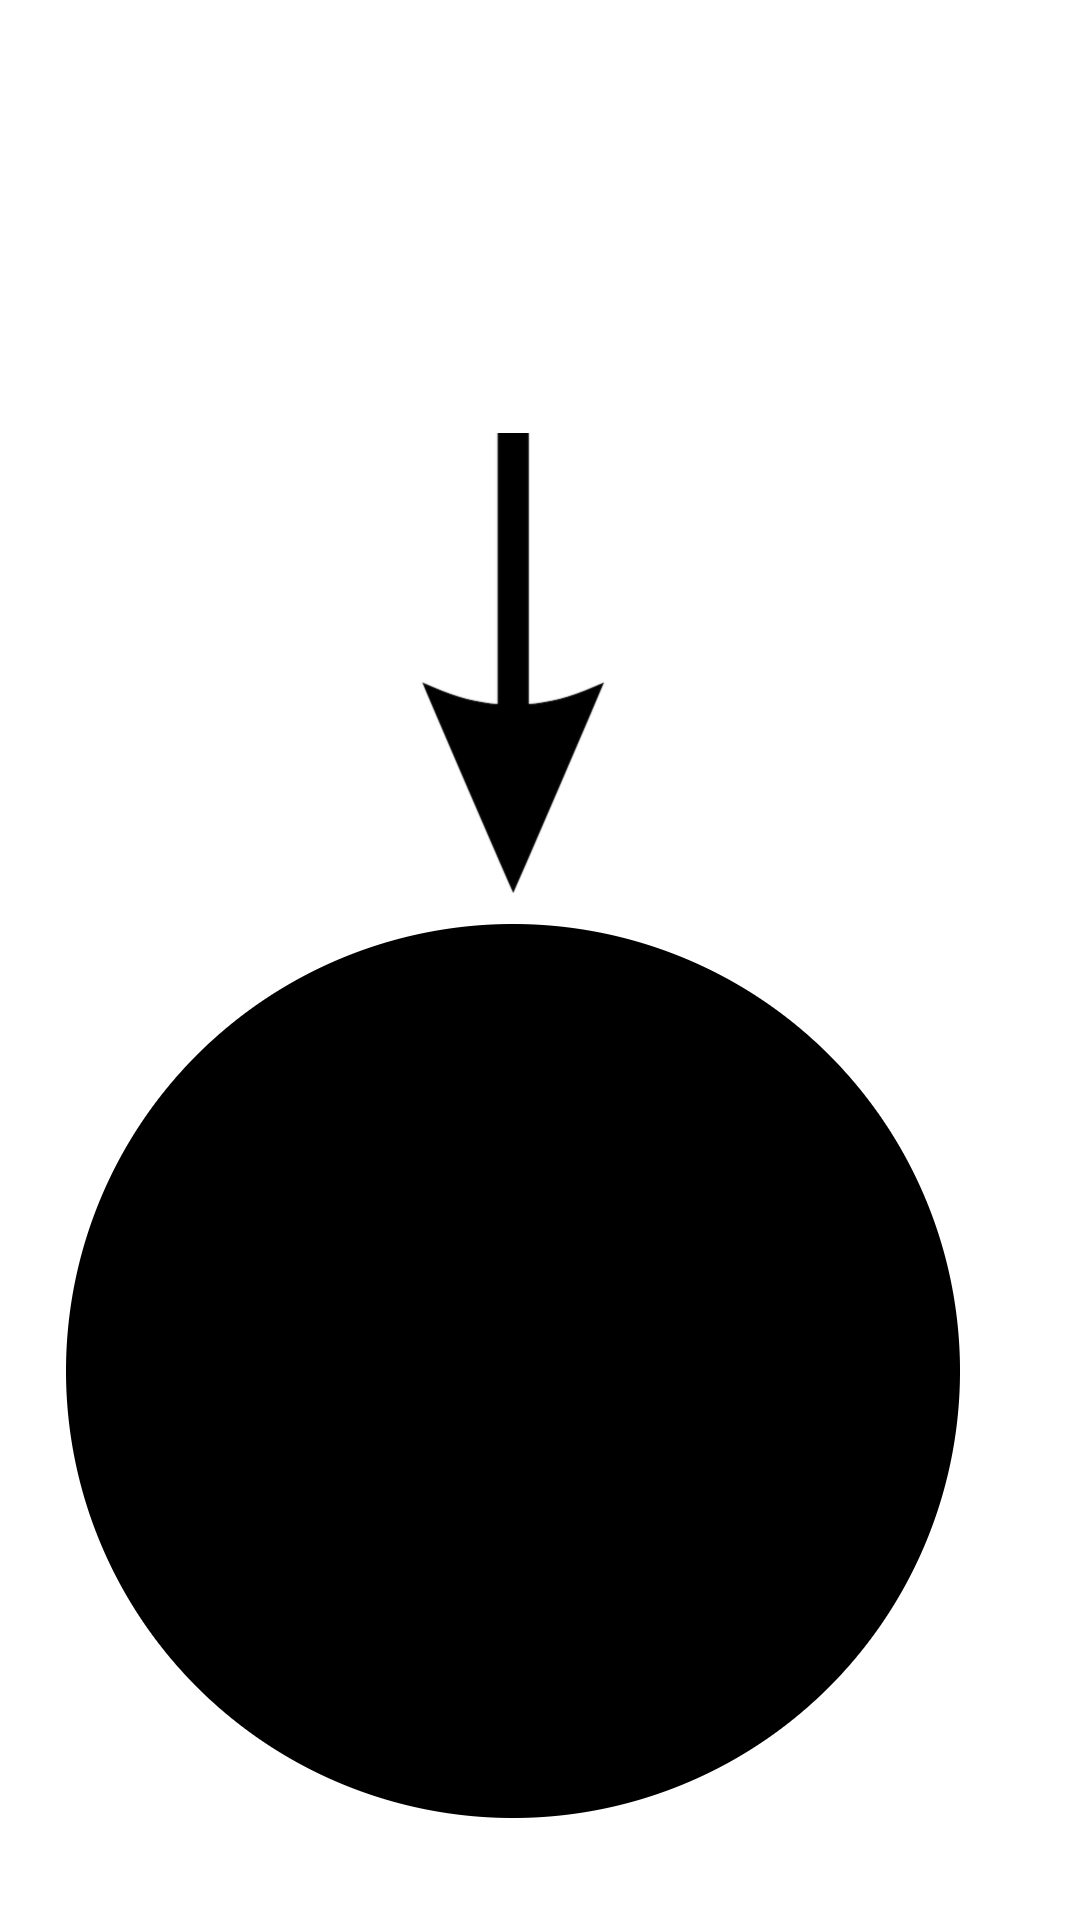
\includegraphics[scale=0.45]{too_close_1}
		\vspace{0.2cm}
		\caption{Snapshots of working algorithm}
	\end{figure}
	}
	\only<2>{
		\begin{figure}
			\centering
			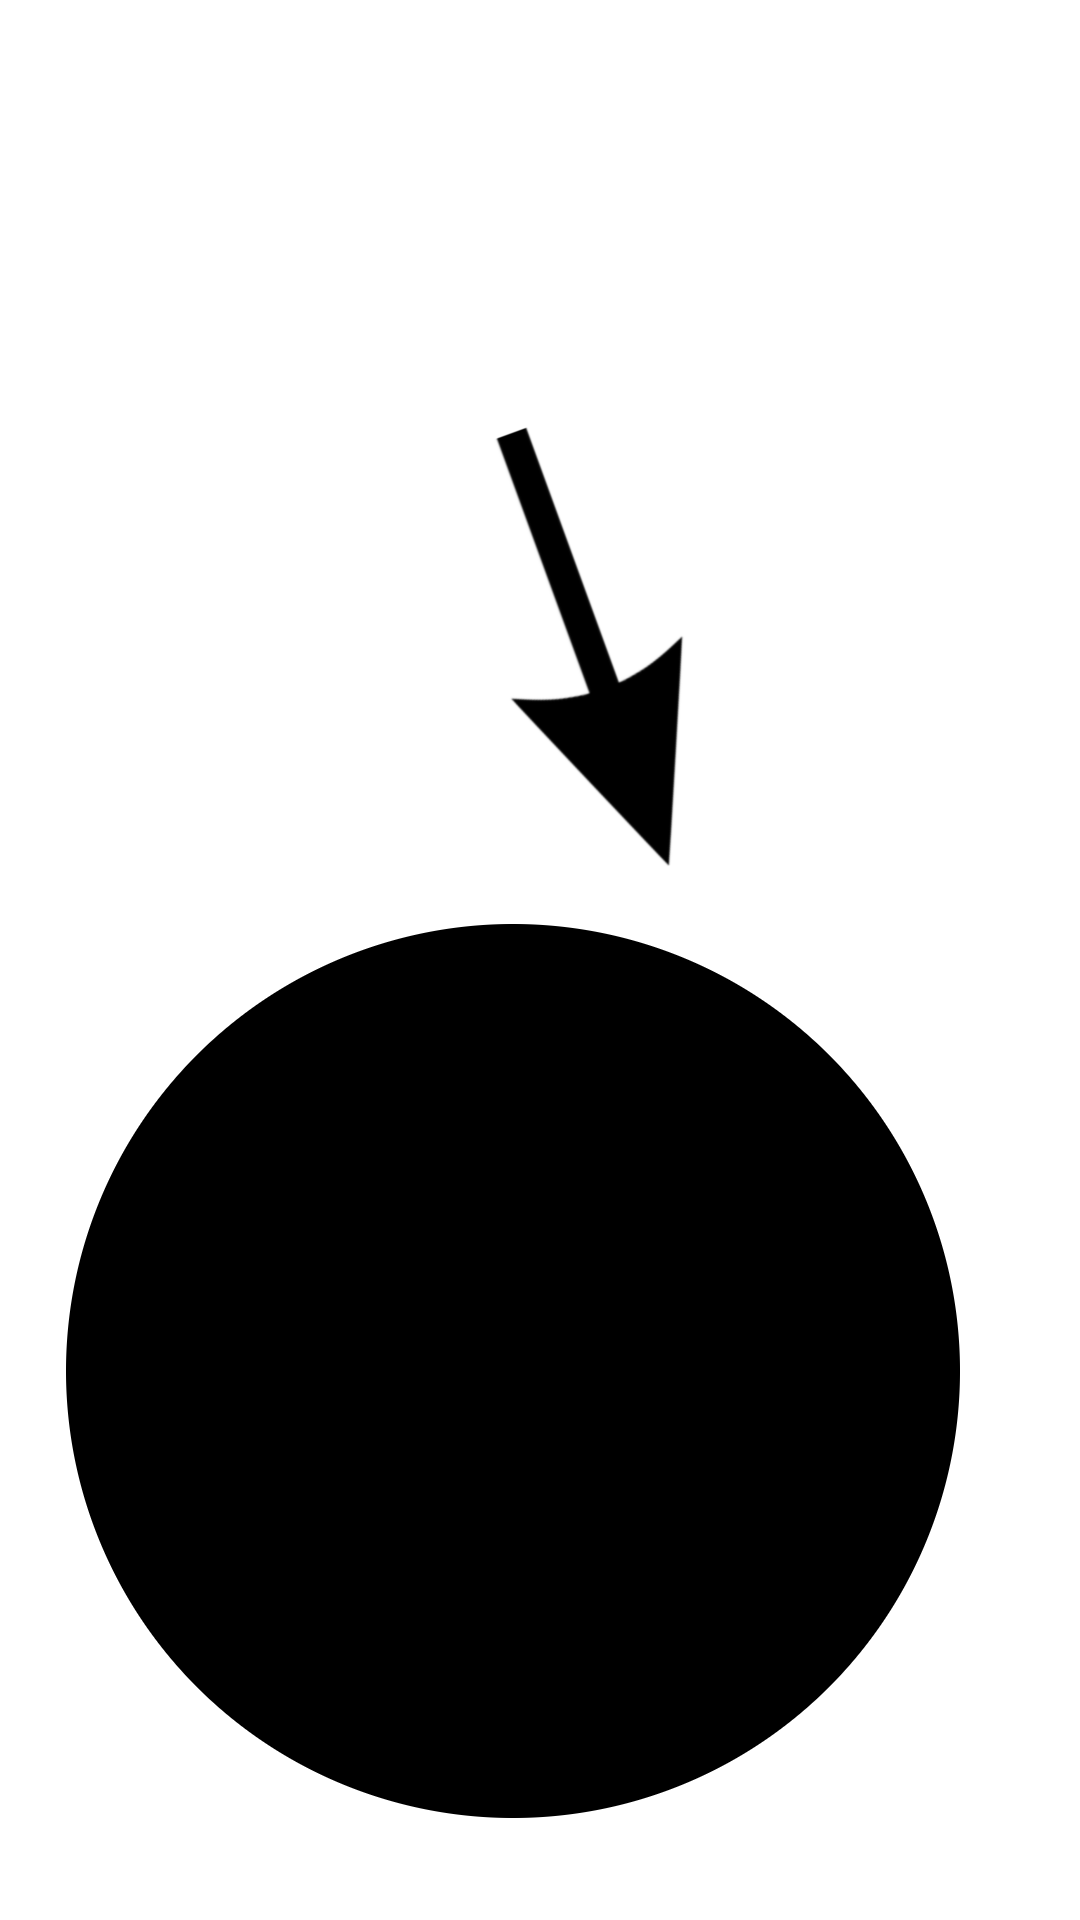
\includegraphics[scale=0.45]{too_close_2}
			\vspace{0.2cm}
			\caption{Snapshots of working algorithm}
		\end{figure}
	}
	\only<3>{
		\begin{figure}
			\centering
			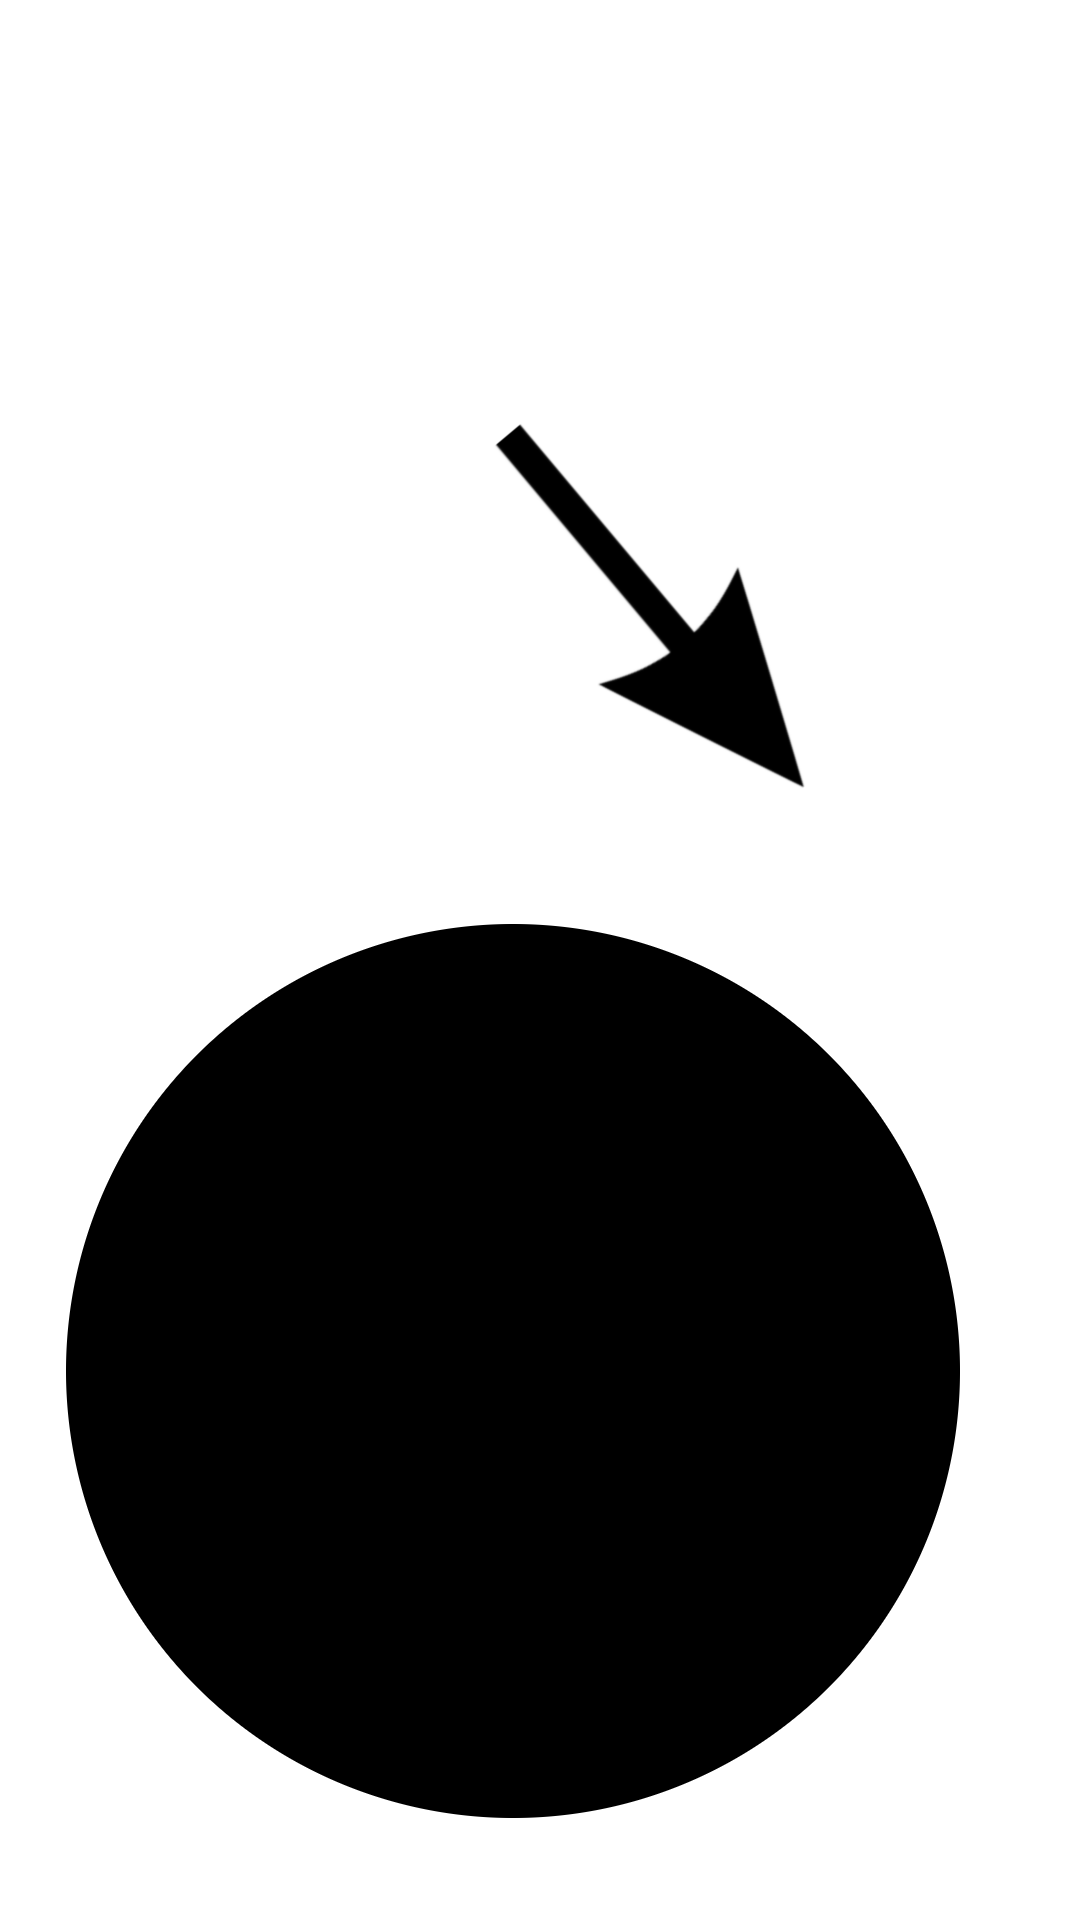
\includegraphics[scale=0.45]{too_close_3}
			\vspace{0.2cm}
			\caption{Snapshots of working algorithm}
		\end{figure}
	}
	\only<4>{
		\begin{figure}
			\centering
			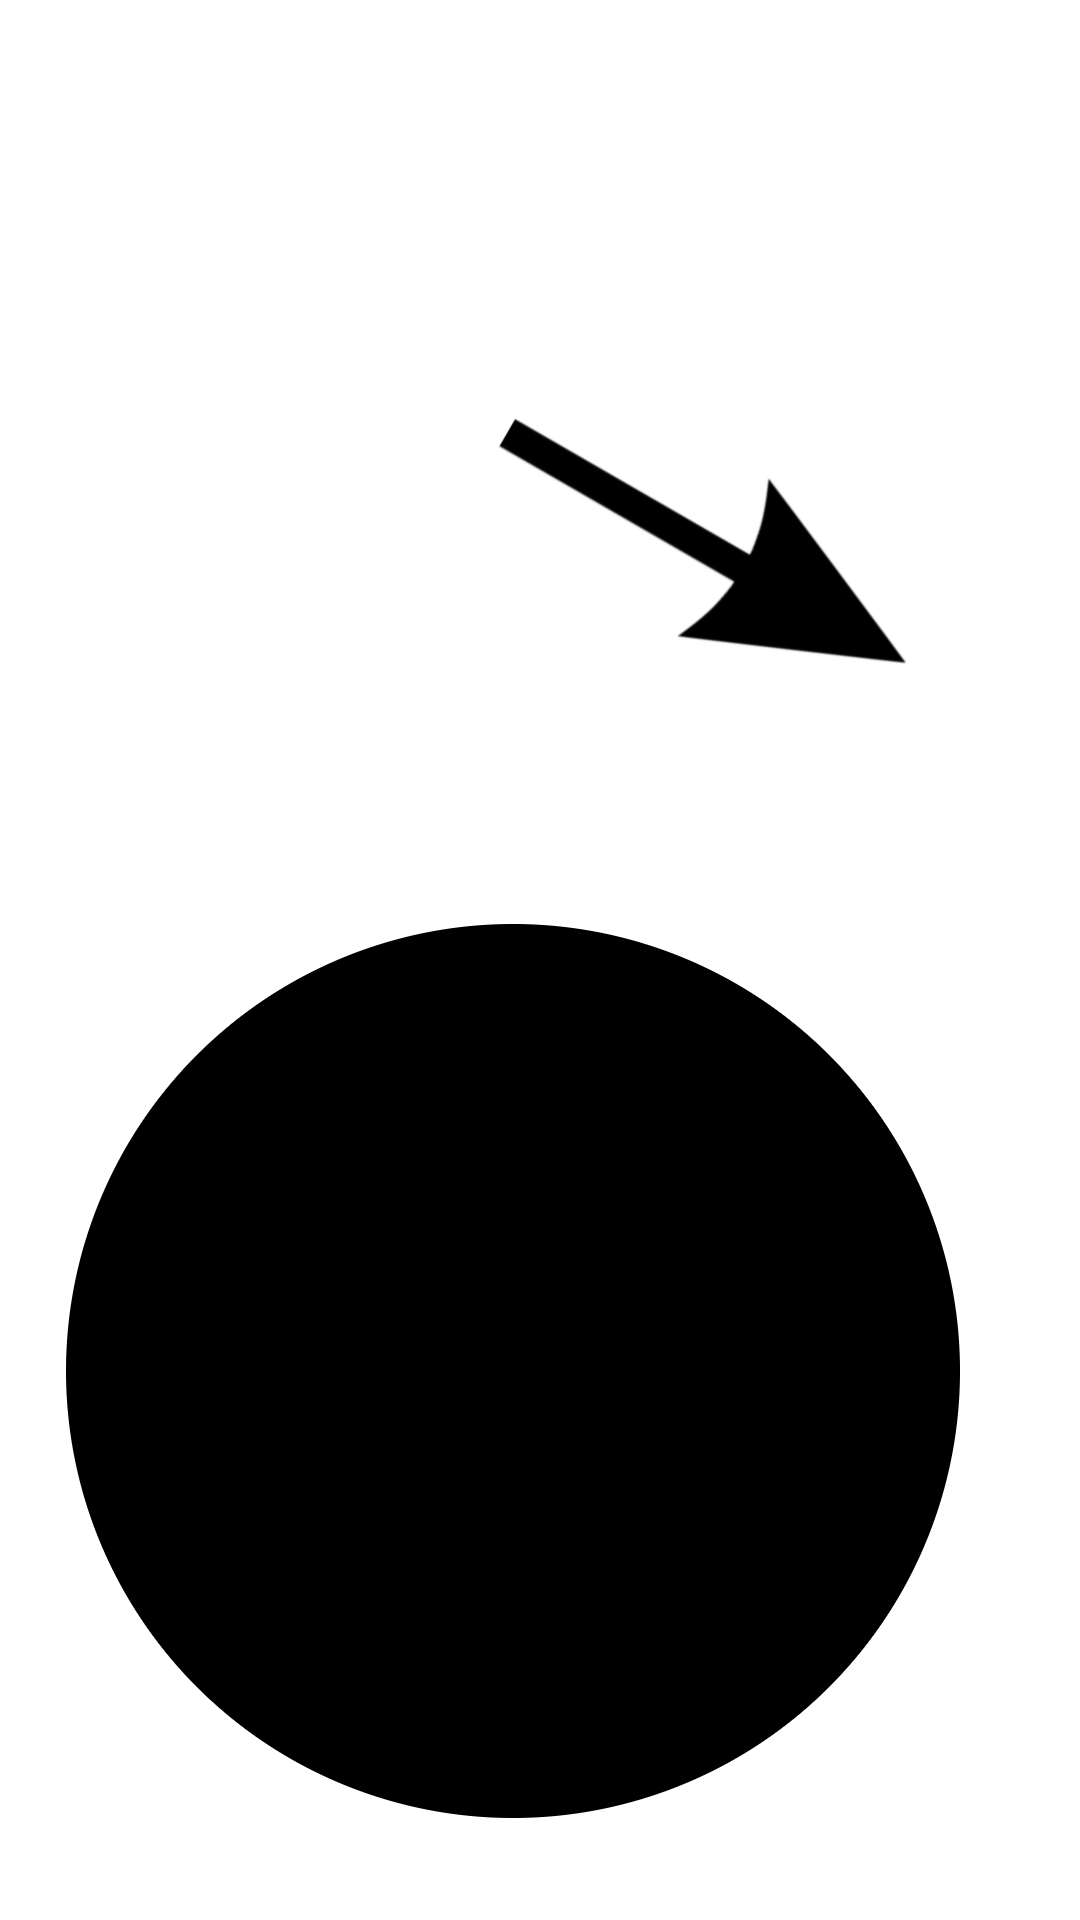
\includegraphics[scale=0.45]{too_close_4}
			\vspace{0.2cm}
			\caption{Snapshots of working algorithm}
		\end{figure}
	}
	\only<5>{
		\begin{figure}
			\centering
			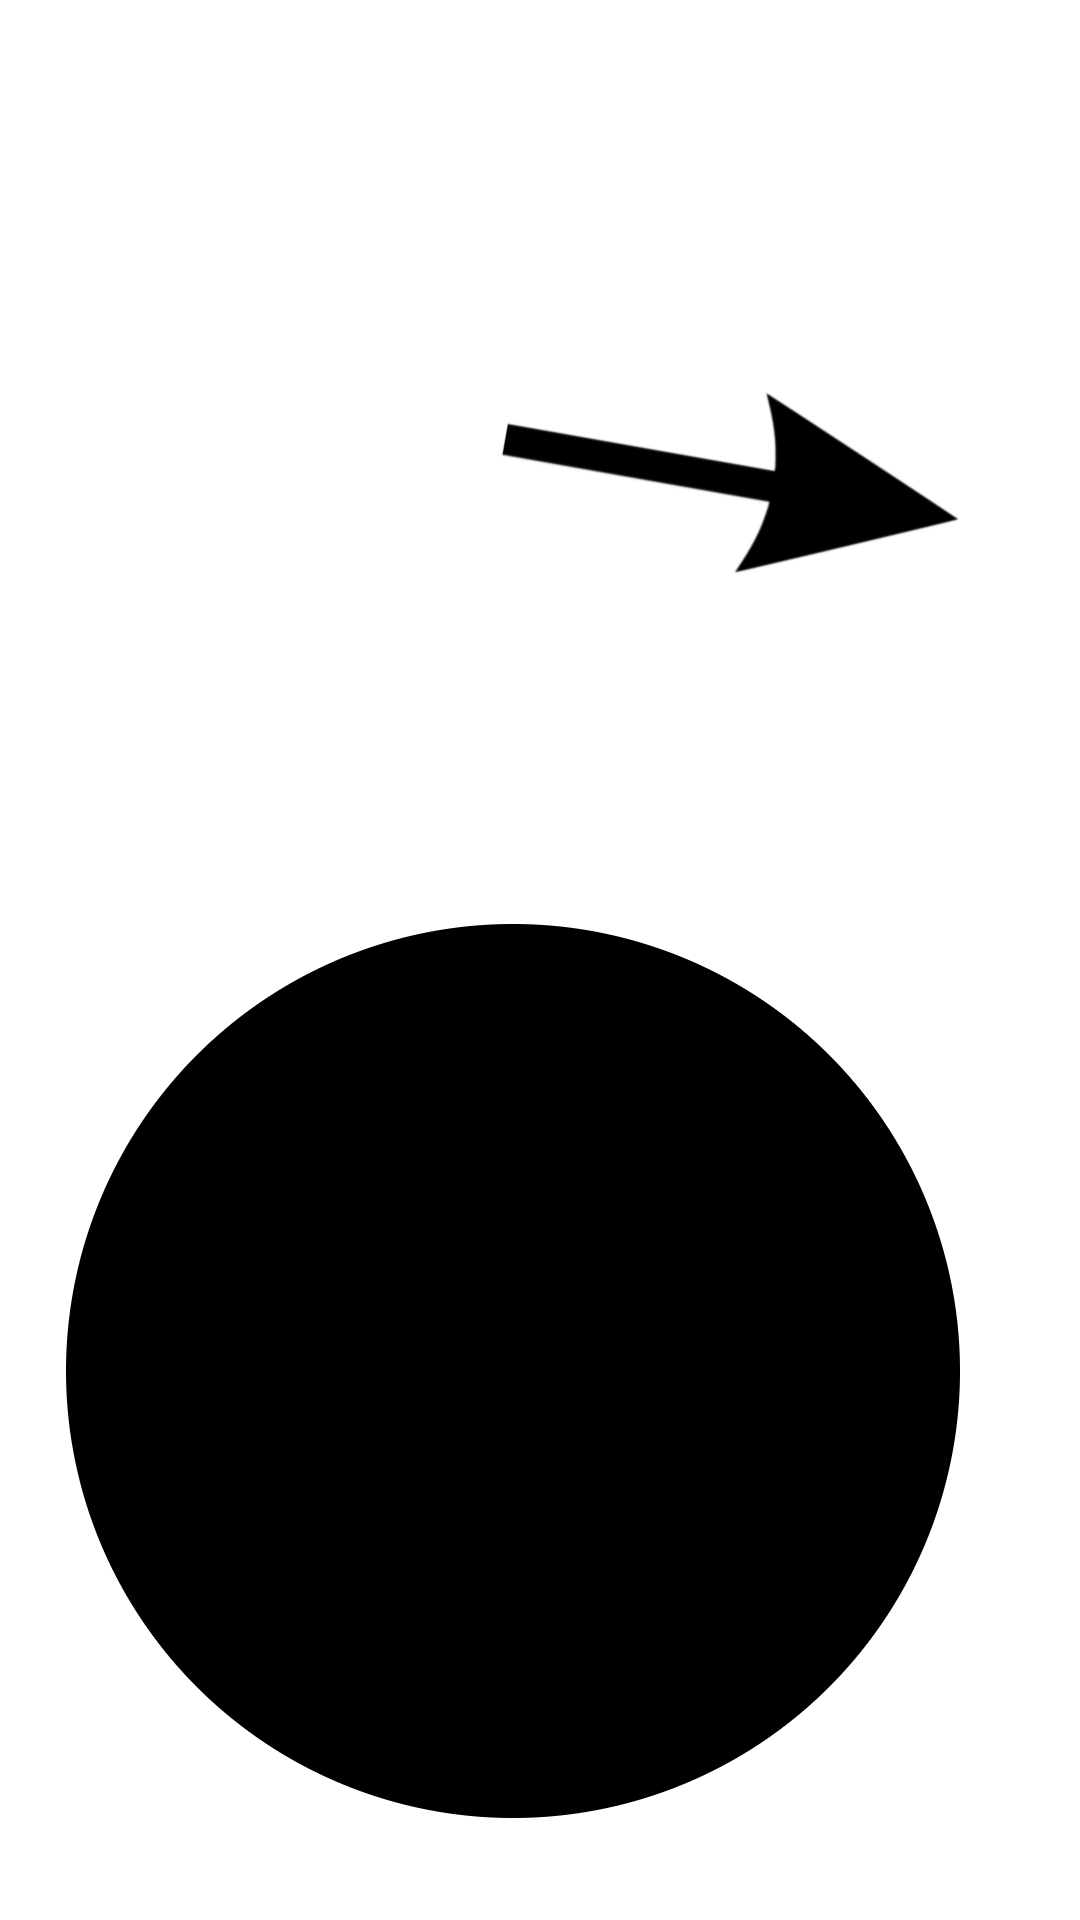
\includegraphics[scale=0.45]{too_close_5}
			\vspace{0.2cm}
			\caption{Snapshots of working algorithm}
		\end{figure}
	}
	\only<6>{
		\begin{figure}
			\centering
			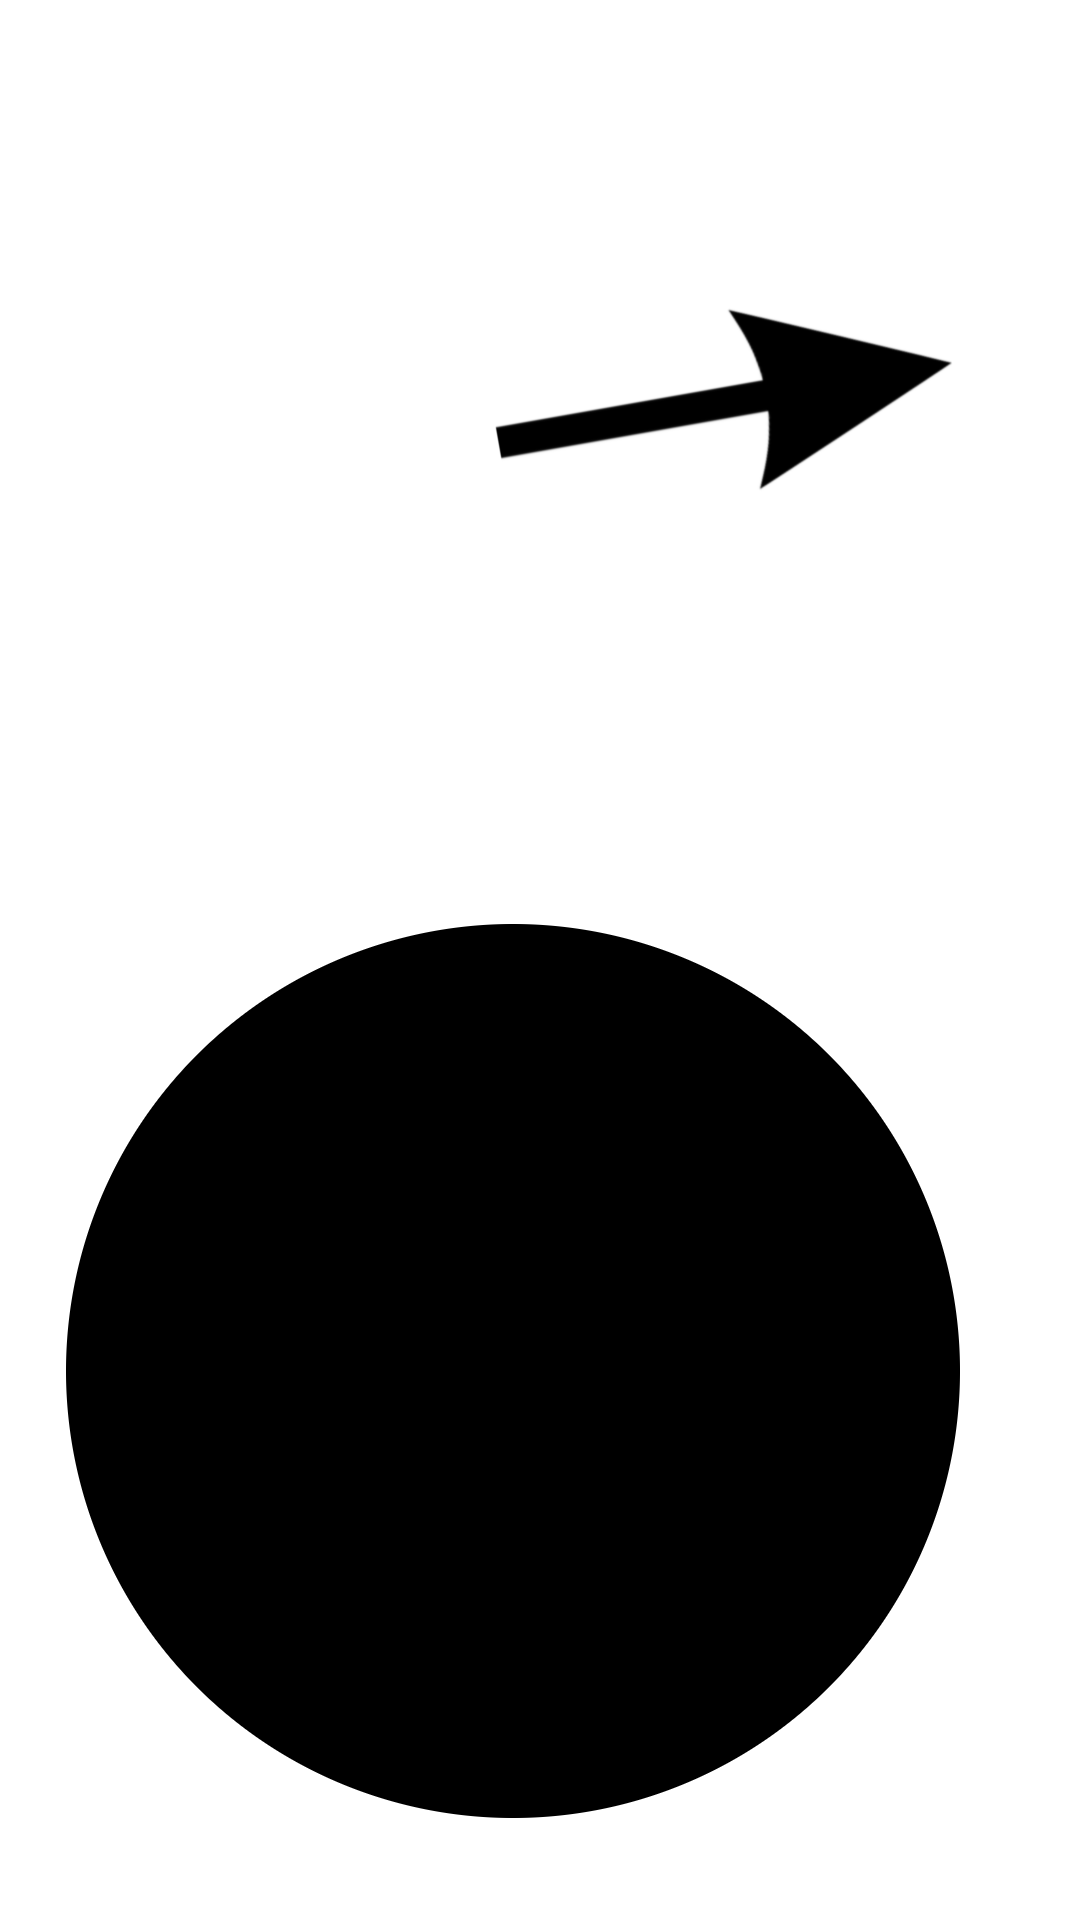
\includegraphics[scale=0.45]{too_close_6}
			\vspace{0.2cm}
			\caption{Snapshots of working algorithm}
		\end{figure}
	}
	\only<7>{
		\begin{figure}
			\centering
			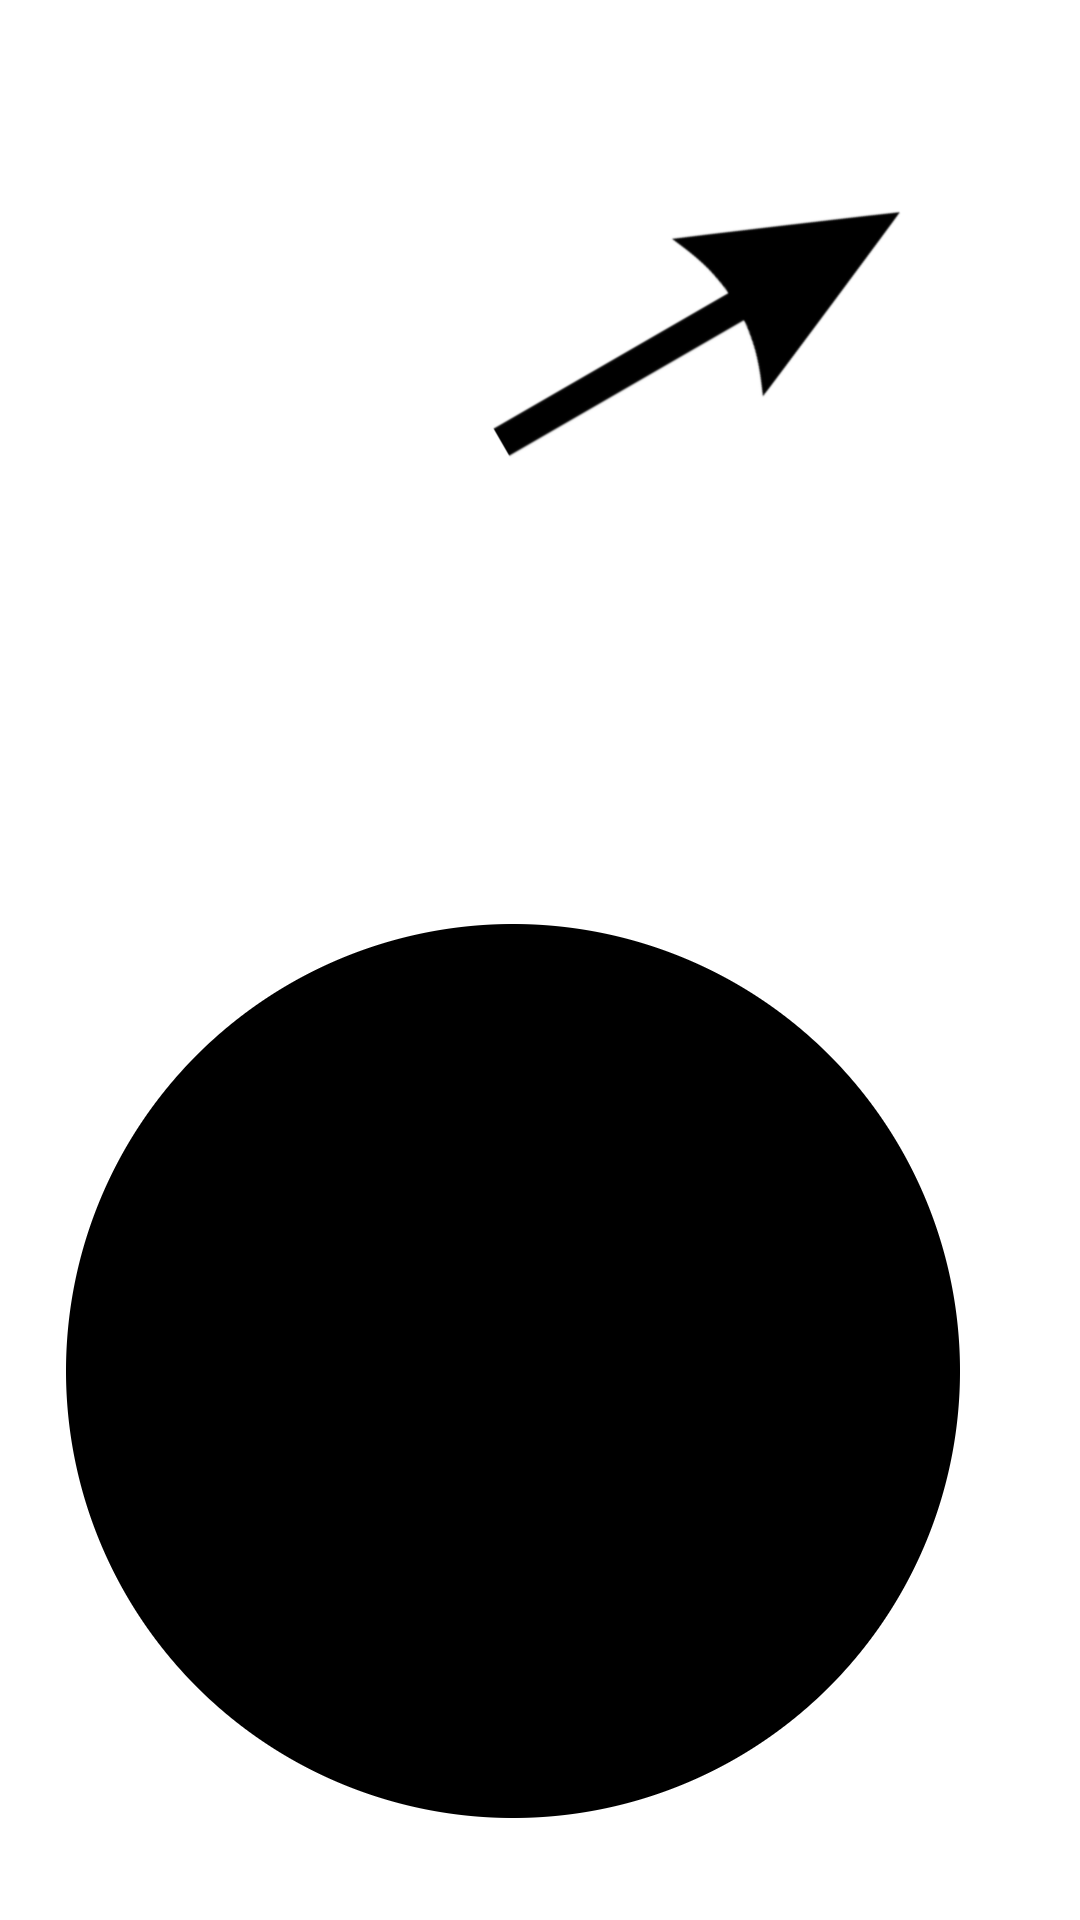
\includegraphics[scale=0.45]{too_close_7}
			\vspace{0.2cm}
			\caption{Snapshots of working algorithm}
		\end{figure}
	}
	\only<8>{
		\begin{figure}
			\centering
			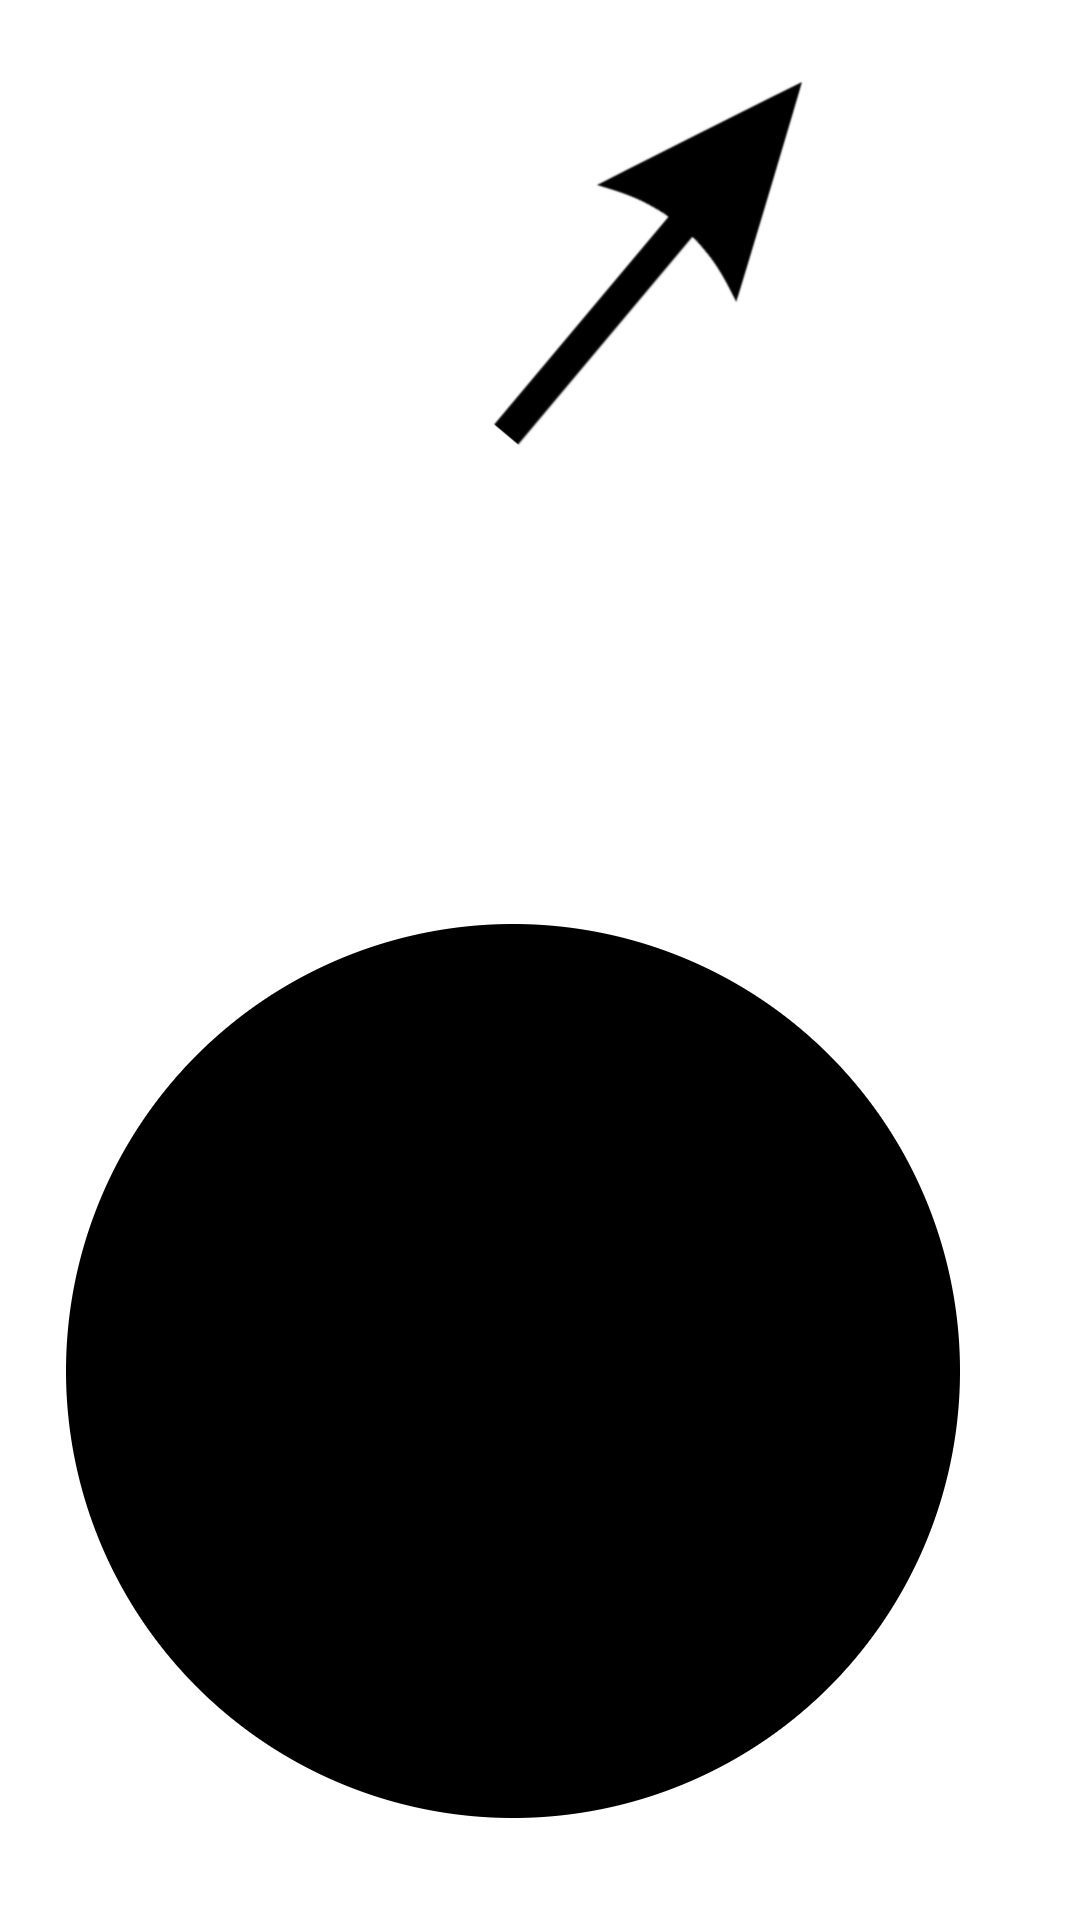
\includegraphics[scale=0.45]{too_close_8}
			\vspace{0.2cm}
			\caption{Snapshots of working algorithm}
		\end{figure}
	}
	\only<9>{
		\begin{figure}
			\centering
			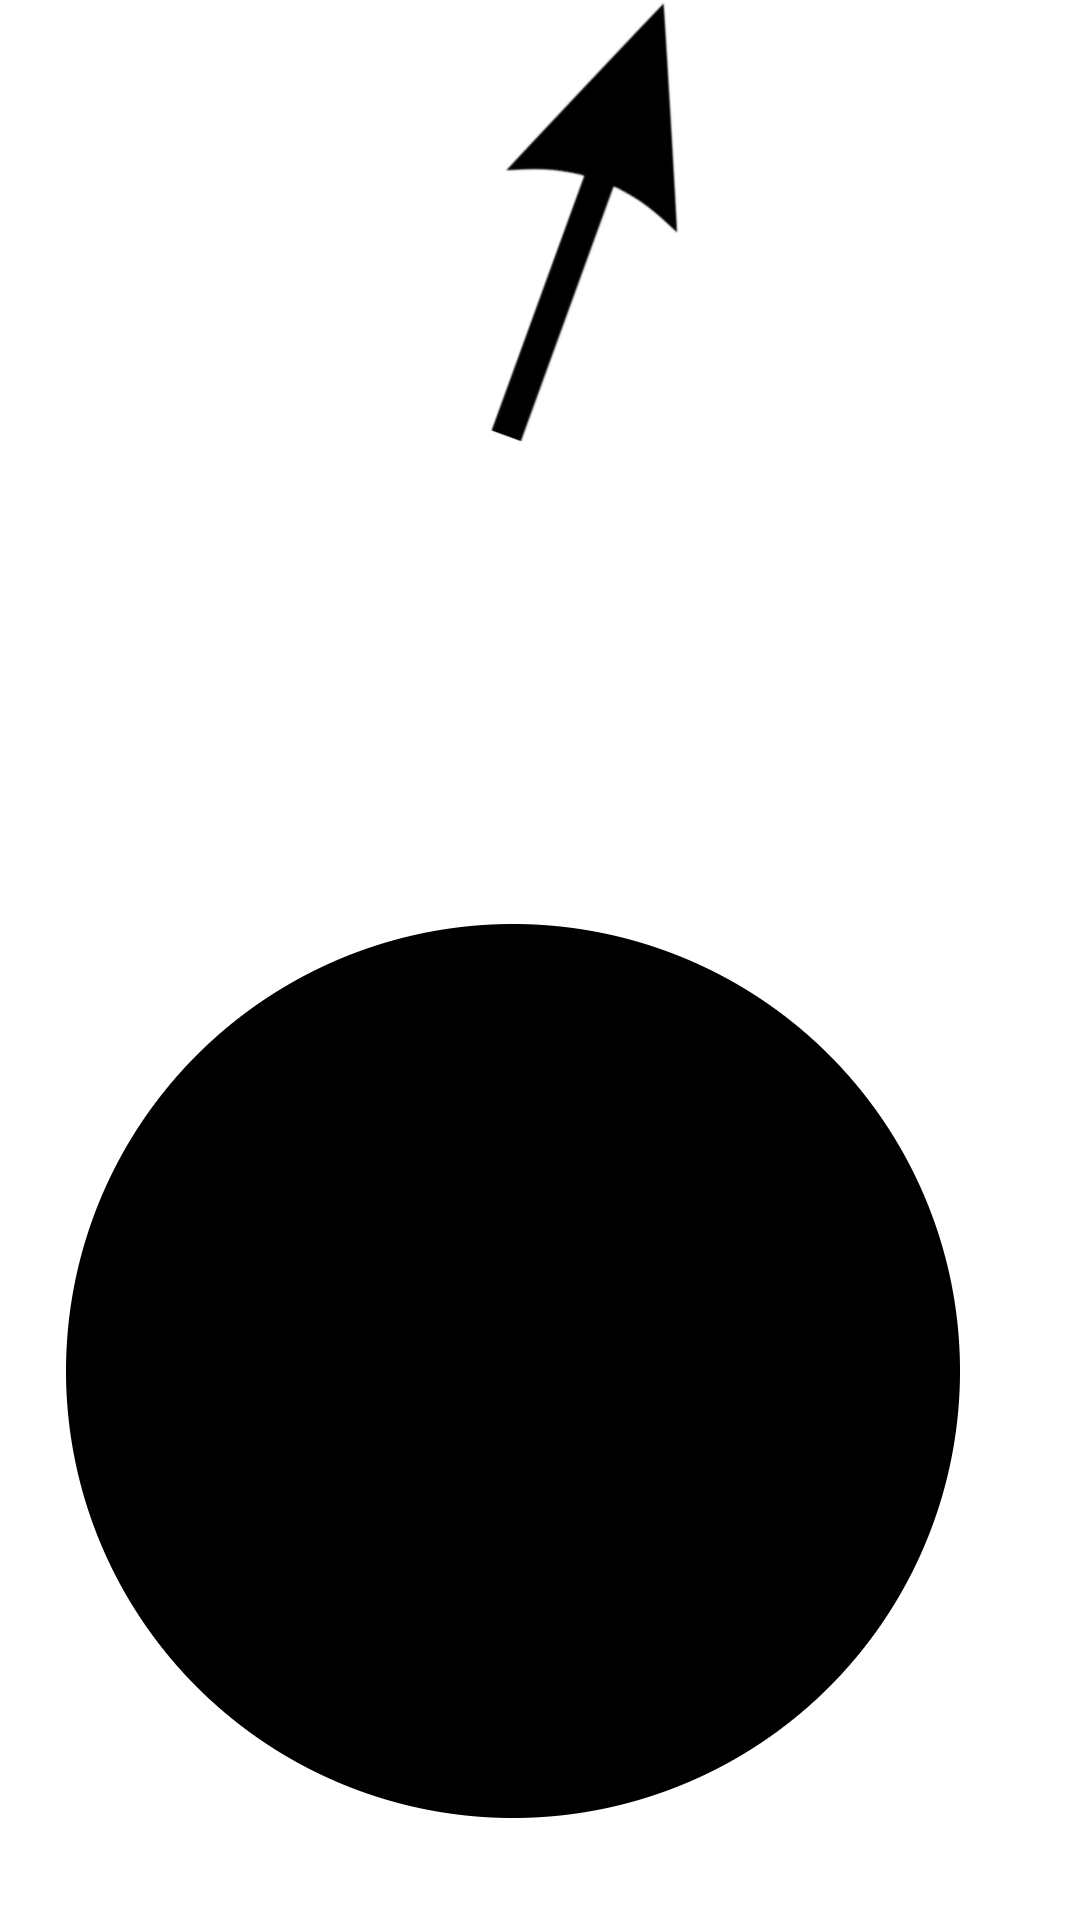
\includegraphics[scale=0.45]{too_close_9}
			\vspace{0.2cm}
			\caption{Snapshots of working algorithm}
		\end{figure}
	}
\end{frame}

\begin{frame}
\frametitle{Flowchart}
\begin{figure}[H]
	\centering
	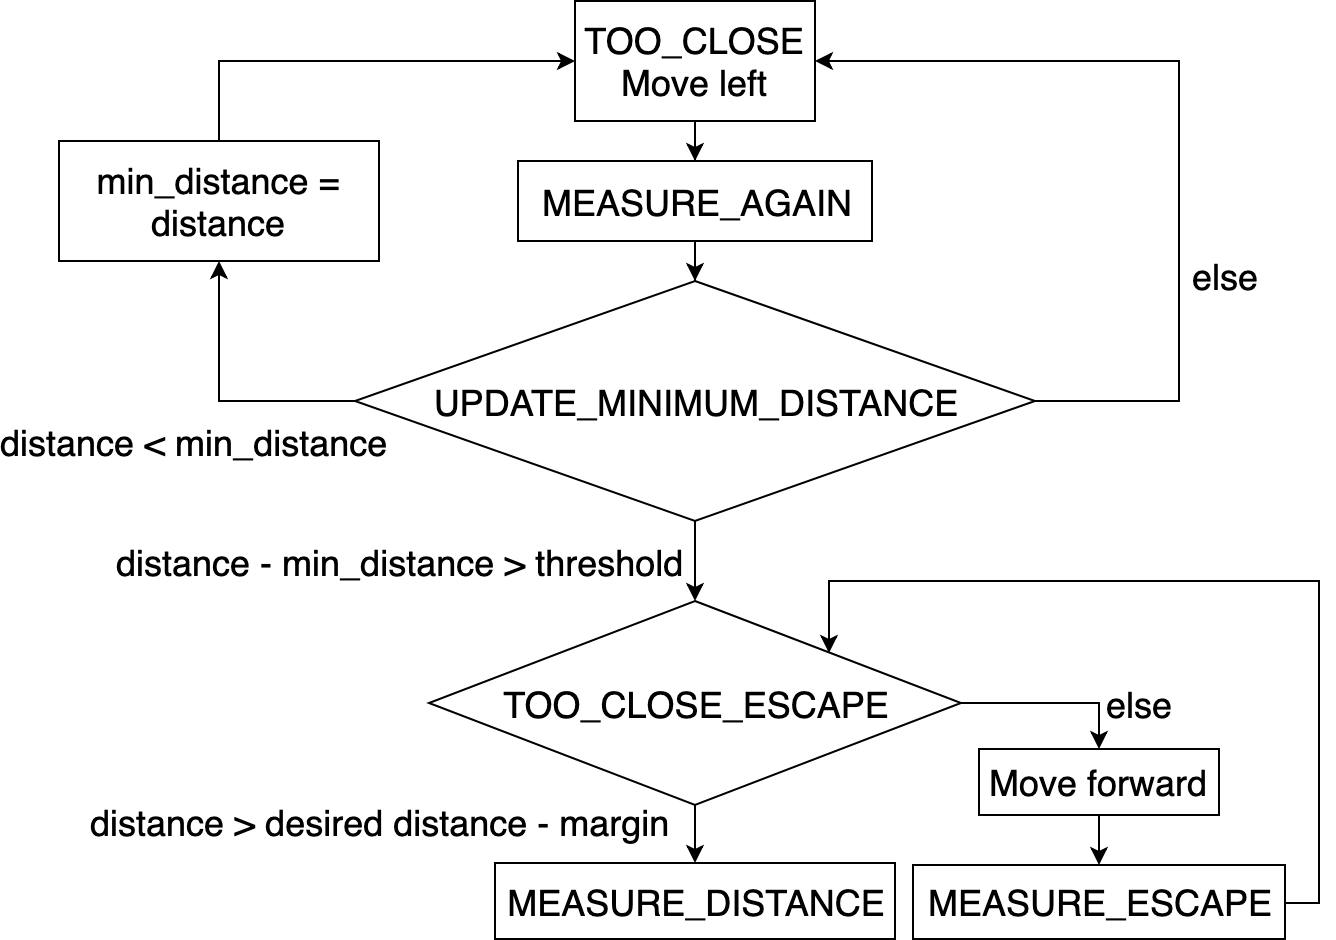
\includegraphics[scale=0.22]{star_planet_escape_compressed_2}
\end{figure}
\end{frame}

\begin{frame}
\frametitle{Efficient orbiting using FSM}
\framesubtitle{Demonstration}
\begin{figure}[H]
	\begin{center}
	\fbox{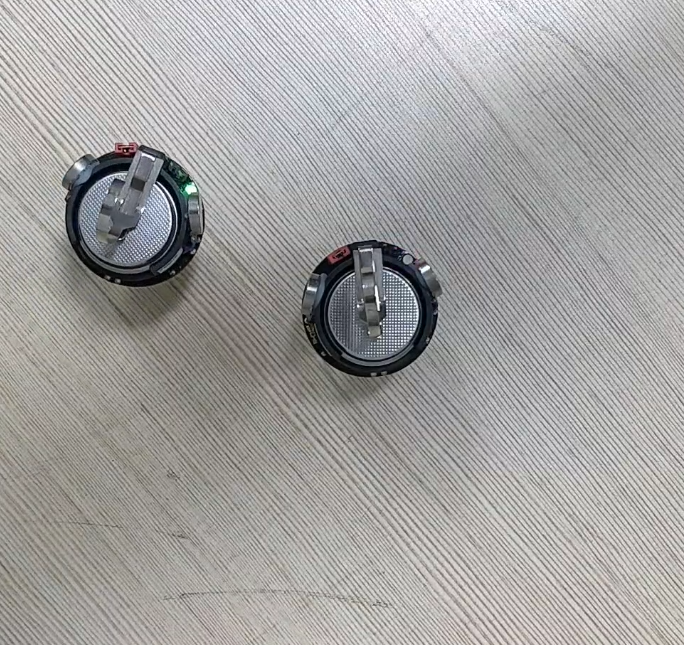
\includegraphics[width=2in]{orbit_after_escape}}\\
	\vspace{0.4cm}
	\caption{\href{https://youtu.be/X6dGCLT0ho8}{Escaping too close region of star by planet followed by orbiting}}
	\label{fig:shape_formation_demo}
	\end{center}
\end{figure}
\end{frame}